\documentclass[a4paper]{article}
\usepackage{amsmath,amsfonts,amssymb}
\usepackage[utf8]{inputenc}
\usepackage{graphicx}
\usepackage{verbatim}
\usepackage{float}
\usepackage[makeroom]{cancel} %
\usepackage[english]{babel}
\usepackage{textcomp}
\usepackage{gensymb} %
\usepackage{color}
\usepackage{subcaption}
\usepackage{caption}
%\usepackage{hyperref}
%\usepackage{physics}
%\usepackage{dsfont}
%\usepackage{amsfonts}
\usepackage{listings}
\usepackage{multicol}
\usepackage{units}
\usepackage{bm}

% From Eirik's .tex
\usepackage{epstopdf}
\usepackage{cite}
\usepackage{braket}
\usepackage{url}
\bibliographystyle{unsrt}

\usepackage{algorithmicx}
\usepackage{algorithm}% http://ctan.org/pkg/algorithms
\usepackage{algpseudocode}% http://ctan.org/pkg/algorithmicx

\usepackage[margin=1cm]{caption}
\usepackage[outer=1.2in,inner=1.2in]{geometry}
% For writing full-size pages
%\usepackage{geometry}
%\geometry{
%  left=5mm,
%  right=5mm,
%  top=5mm,
%  bottom=5mm,
%  heightrounded,
%}

% Finding overfull \hbox
\overfullrule=2cm

\lstset{language=IDL}
 %\lstset{alsolanguage=c++}
\lstset{basicstyle=\ttfamily\small}
 %\lstset{backgroundcolor=\color{white}}
\lstset{frame=single}
\lstset{stringstyle=\ttfamily}
\lstset{keywordstyle=\color{red}\bfseries}
\lstset{commentstyle=\itshape\color{blue}}
\lstset{showspaces=false}
\lstset{showstringspaces=false}
\lstset{showtabs=false}
\lstset{breaklines}
\lstset{aboveskip=20pt,belowskip=20pt}

\lstset{basicstyle=\footnotesize, basewidth=0.5em}
\lstdefinestyle{cl}{frame=none,basicstyle=\ttfamily\small}
\lstdefinestyle{pr}{frame=single,basicstyle=\ttfamily\small}
\lstdefinestyle{prt}{frame=none,basicstyle=\ttfamily\small}
% \lstinputlisting[language=Python]{filename}


\definecolor{codepurple}{rgb}{0.58,0,0.82}
\definecolor{backcolour}{rgb}{0.95,0.95,0.92}
\definecolor{dkgreen}{rgb}{0,0.6,0}
\definecolor{gray}{rgb}{0.5,0.5,0.5}
\definecolor{magenta}{rgb}{0.58,0,0.82}

\lstdefinestyle{pystyle}{
  language=Python,
  aboveskip=3mm,
  belowskip=3mm,
  columns=flexible,
  basicstyle={\small\ttfamily},
  backgroundcolor=\color{backcolour},
  commentstyle=\color{dkgreen},
  keywordstyle=\color{magenta},
  numberstyle=\tiny\color{gray},
  stringstyle=\color{codepurple},
  basicstyle=\footnotesize,
  breakatwhitespace=false,
  breaklines=true,
  captionpos=b,
  keepspaces=true,
  numbers=left,
  numbersep=5pt,
  showspaces=false,
  showstringspaces=false,
  showtabs=false,
  tabsize=2
}

\lstset{language=[90]Fortran,
  basicstyle=\small\ttfamily,
  keywordstyle=\color{red},
  commentstyle=\color{blue},
  stringstyle=\color{dkgreen},
  morecomment=[l]{!\ },
  numbers=left,
  numbersep=5pt
}

%%%%%%%%%%%%%%%%%%%%%%%%%%%%%%%%
% Self made macros here yaaaaaay
\newcommand\answer[1]{\underline{\underline{#1}}}
\newcommand\pd[2]{\frac{\partial #1}{\partial #2}}
\newcommand\red[1]{\textcolor{red}{\textbf{#1}}}
\newcommand\numberthis{\addtocounter{equation}{1}\tag{\theequation}}
% Usage: \numberthis \label{name}
% Referencing: \eqref{name}

% Some matrices
\newcommand\smat[1]{\big(\begin{smallmatrix}#1\end{smallmatrix}\big)}
\newcommand\ppmat[1]{\begin{pmatrix}#1\end{pmatrix}}

%%%%%%%%%%%%%%%%%%%%%%%%%%%%%%%%%
% Eirik's self made macros
\newcommand{\s}{^{*}}
\newcommand{\V}[1]{\mathbf{#1}}
\newcommand{\husk}[1]{\color{red} #1 \color{black}}
\newcommand{\E}[1]{\cdot 10^{#1}}
\newcommand{\e}[1]{\ \text{#1}}
\newcommand{\tom}[1]{\big( #1 \big)}
\newcommand{\Tom}[1]{\Big( #1 \Big)}
\newcommand{\tomH}[1]{\big[ #1 \big] }
\newcommand{\TomH}[1]{\Big[ #1 \Big]}
\newcommand{\tomK}[1]{ \{ #1 \} }
\newcommand{\TomK}[1]{\Big\lbrace #1 \Big\rbrace}
\newcommand{\bigabs}[1]{\left| #1 \right|}

% Practical macros for FYS-STK4155
\newcommand{\XX}{\mathbf{X}}
\newcommand{\II}{\textbf{I}}
\newcommand{\T}{\mathsf{T}}

% Section labeling
%\usepackage{titlesec}% http://ctan.org/pkg/titlesec
%\renewcommand{\thesubsection}{\arabic{subsection}}

% Title/name/date
\title{FYS-STK4155: Project 1}
\author{Simen Nyhus Bastnes}
\date{5. October 2020}

\begin{document}
\maketitle
%%%%%%%%%%%%%%%%%%%%%%%%%%%%%%%%%%%%%%%%%%%%%%%%%
\begin{abstract}
In this project, we will study various methods of linear regression, namely the Ordinary Least Squares method, Ridge, and Lasso regression, as well as investigate resampling the data via Bootstrapping and $k$-fold Cross-Validation. The data we will be looking at is the so-called Franke function, as well as terrain elevation data from a region in Norway. The Franke function gives us a way of testing our implementation before moving on to the more complex terrain data.%The goal of this project is to do linear regression with bootstrapping and cross-validation on the Franke function and real data.
\end{abstract}
%%%%%%%%%%%%%%%%%%%%%%%%%%%%%%%%%%%%%%%%%%%%%%%%%%%%%%%%%%%%%%%%%%%%%%%%%%%%%%%%%%%%%%%%%%
%%%%%%%%%%%%%%%%%%%%%%%%%%%%%%%%%%%%%%%%%%%%%%%%%%%%%%%%%%%%%%%%%%%%%%%%%%%%%%%%%%%%%%%%%%
\section{Introduction}
% not good enough maybe check first sentence

With the emergence of more powerful computers, the field of machine learning is steadily becoming an integral part of both business and many fields of science. While many of the concepts and algorithms used in machine learning today has been known for a long time, some of them have simply been too computationally expensive to do efficiently. While not typically too computationally heavy \red{do something about this}, linear regression is one of the simplest and most-studied forms of machine learning, and provides a good introduction to concepts commonly used in machine learning. 
\\\\
In this project, we will look at three different methods of regression analysis and compare how they fare against each other. The methods we will be using is the Ordinary Least Squares method, Ridge regression, and Lasso regression. We will also see how resampling the data affects the results from the regression methods, by implementing the Bootstrap algorithm and the $k$-fold Cross-Validation.
\\\\
There are two different data sets that will be studied in this project. The first, is the Franke function from \cite{Franke}, as well as terrain data for a region in Norway taken from \cite{terrain}. First, in Chapter \ref{chap:theory} we will introduce the theory behind linear regression, as well as the the regression methods and resampling methods employed later in the project. In Chapter \ref{chap:implement} we go through the implementation of the methods, explaining how the code is structured and used. Then, in Chapter \ref{chap:results} we go through the results of both the Franke function and the terrain data, while discussing them. %discussing them in more detail in Chapter \ref{chap:discussion}. 
Lastly, we conclude our findings in Chapter \ref{chap:conclusion}.

%%%%%%%%%%%%%%%%%%%%%%%%%%%%%%%%%%%%%%%%%%%%%%%%%%%%%%%%%%%%%%%%%%%%%%%%%%%%%%%%%%%%%%%%%%
%%%%%%%%%%%%%%%%%%%%%%%%%%%%%%%%%%%%%%%%%%%%%%%%%%%%%%%%%%%%%%%%%%%%%%%%%%%%%%%%%%%%%%%%%%
\section{Theory} \label{chap:theory}
%For the derivation of the OLS method, Ridge, and Lasso regression, we will follow Chapter 2.3 and 3.4 of Hastie et al. \cite{Hastie}
\subsection{Linear regression} \label{sec:linreg}
%Assume we have a data set $\bm{y}$
%At its core, x
Linear regression is a method of fitting a set of $p$ \textit{predictors} $\bm{X}$ to a data set $\bm{y}$, while minimizing the error between the \textit{response} $\bm{\tilde y}$ and the actual data $\bm{y}$. For each of the $n$ samples $y_i$ in the data set the relationship between the response and the predictors $\bm{X}_i$ is modeled in a linear fashion, giving us the following matrix equation
\begin{align*}
	\mathbf{y} &= \XX\beta + \bm{\epsilon}
\end{align*}
where $\beta = (\beta_0, \beta_1, ..., \beta_ {p-1})^\T$ are the regression parameters we are trying to estimate, one for each predictor, and $\bm{\epsilon}$ is the error in our approximation. The matrix $\XX$ is often called the design matrix, and the equation can be written a bit more explicitly as
\begin{align*}
	y_i &= \beta_0 + X_{i,1}\beta_1 + ... + X_{i,p-1}\beta_{p-1} + \epsilon_i
\end{align*}
Exactly what each predictor is can vary a lot from case to case, and how the design matrix is set up is important for the accuracy of the fit. In our case, we will focus on a form of linear regression where the predictors is on the form of a polynomial in the input parameters. In the case where we have a data set $\bm{y}(\bm{x})$, the design matrix can for example be written on the form of
\begin{align*}
	\XX &= (\bm{x}^0, \bm{x}^1, ... , \bm{x}^{p-1})
\end{align*} 
With that said, we still need some way to find the $\beta$'s that fit the data best, and we will now look at three ways to try to do this.
% This is done
%Assuming that we have a set of \textit{response} allalal
%linear regresssion Fitting a continuous function with linear parameterization in terms of the parameters $\beta$.
%Giving us the matrix equation
%Linear regression is a way of modeling a relationship between the response $y_i$ and some amount of explanatory variables $x_i$ in a linear fashion. Assume we have 
%\begin{align*}
%	\mathbf{y} &= \beta_0 + \sum_{i=1}^{p}\XX_i\beta_i + \mathbf{\varepsilon}_i
%	\mathbf{y} &= \XX\beta + \mathbf{\varepsilon}\\
%	\mathbf{y}_i &= \beta_0 + \sum_{j=1}^{p}\XX_{ij}\beta_j + \mathbf{\varepsilon}_i	
%\end{align*}

\subsubsection{Ordinary least squares}
Following Chapter 2.3 of Hastie et al. \cite{Hastie}, in order to find the optimal regression parameters $\beta$, the OLS method minimizes the residual sum of squares
\begin{align*}
	\text{RSS}(\beta) &= \sum_{i=1}^N(y_i-x_i^T\beta)^2
\end{align*}
With $\bm{y}$ as the vector containing all $N$ $y_i$, and $X$ an $N\times p$ matrix as shown in section \ref{sec:linreg}, this can be written as
\begin{align*}
	\text{RSS}(\lambda) &= (\bm{y} - \XX\beta)^\T(\bm{y}-\XX\beta)
\end{align*}
Differentiating with respect to $\beta$ we get
\begin{align*}
	\pd{\text{RSS}}{\beta} &= X^\T(\bm{y}-\XX\beta)
\end{align*}
In order to find an optimal $\beta$, this has to be zero
\begin{align*}
	\XX^\T(\bm{y}-\XX\beta) &= 0\\
	\XX^\T\XX\beta &= \XX^T\bm{y}
\end{align*}
Finally giving us the expression for the optimal regression parameters
\begin{align*}
	\beta &= (\XX^\T\XX)^{-1}\XX^\T\bm{y}
\end{align*}
assuming that $\XX^\T\XX$ is invertible.

\subsubsection{Ridge regression}
Ridge regression is an example of a so-called shrinkage method, which shrinks the regression coefficients by adding a small penalty proportional to their size.
\begin{align*}
	\beta^{\text{Ridge}} &= \underset{\beta\in \mathbb{R}^{p}}{\text{min}}\frac{1}{n}||\bm{X}\beta - \bm{y}||^2_2 + \lambda||\beta||^2_2
\end{align*}
where $\lambda$ is a regularization parameter that controls the amount of shrinkage, and we $||\beta||^2_2 \leq t$ where $t$ is a finite number larger than zero. The higher $\lambda$, the more shrinkage occurs. This can be shown to give the Ridge solution
\begin{align*}
	\beta^{\text{Ridge}} &= (\XX^\T\XX + \lambda I)^{-1}\XX^\T\bm{y}
\end{align*}
The aim with Ridge regression is to limit the potential problems with singularities when computing the inverse of $\XX^\T\XX$, which can be a problem when there are many correlated variables.
\subsubsection{Lasso regression}
Lasso regression is another shrinkage method, with a slightly different optimization equation compared to Ridge regression
\begin{align*}
	\beta^{\text{Lasso}} &= \underset{\beta\in \mathbb{R}^{p}}{\text{min}}\frac{1}{n}||\bm{X}\beta - \bm{y}||^2_2 + \lambda||\beta||_1
\end{align*}
where $||\beta||_1$ is the $L_{1}$ norm.
\subsection{Bias-Variance decomposition}
\begin{align*}
	C(\XX, \beta) &= \frac{1}{n}\sum_{i=0}^{n-1}(y_i-\tilde y_i)^2 = \mathbb{E}[(\bm{y}-\bm{\tilde y})^2]
\end{align*}
\subsection{R2????}
\subsection{Confidence intervals}
For the OLS and Ridge regression cases, it is possible to derive the variance of $\beta$ (a proper derivation is given in \cite{vanwieringen2020lecture}), and thus the confidence intervals as well. For the OLS method, the variance is given by
\begin{align*}
	\text{Var}(\beta) &= \sigma^2(\XX^\T\XX)^{-1}
\end{align*}
where $\sigma^2$ is the estimated variance of $y$ given by %TODO a eiwahjhlkwa hw
\begin{align*}
	\sigma^2 &= \frac{1}{N-p-1}\sigma_{i=1}^N(y_i-\tilde y_i)^2
\end{align*}
Taking the square root of the diagonal of $(\XX^\T\XX)^{-1}$ gives us an estimate of the variance of the $j$-th regression coefficient
\begin{align*}
	\sigma^2(\beta_j) &= \sigma^2\sqrt{[\XX^\T\XX]^{-1}_{jj}}
\end{align*}
Letting us construct the 95\% confidence intervals by
%The confidence interval is then given by
\begin{align*}
	\text{CI}(\beta_j) &= \bigg[\beta_j - 2\sqrt{\sigma_2(\beta_j)}\:,\;\; \beta_j + 2\sqrt{\sigma_2(\beta_j)}\bigg]
\end{align*}
%Both can be found in van vieringen | also lecture notes...... 36
Similarly, the variance for $\beta$ for Ridge regression can be found to be
\begin{align*}
\text{Var}[\beta^{\text{Ridge}}] &= \sigma^2[\XX^\T\XX + \lambda\II]^{-1}
\XX^\T \XX[(\XX^\T \XX + \lambda \II)^{-1}]^\T
\end{align*}
and confidence interval can be constructed following the same steps as done above for OLS.% the same way as above for OLS.

\subsection{Resampling methods}
In order to assess our models properly, we will be using some form of resampling. Specifically, we will be looking at the Bootstrap, and the standard $k$-fold Cross-validation resampling methods.
\subsubsection{Bootstrap}
The basic concept of the Bootstrap resampling method is to create new data sets by drawing samples (with replacement) from the training data set. Algorithm \ref{alg:bootstrap} shows the Bootstrap method given a data set $\mathcal{L}$ consisting of the data $\XX_{\mathcal{L}} = \{(y_j, \bm{x}_j), j= 0 \,...\, n-1\}$
\begin{algorithm}[H]
\caption{Bootstrap}
\begin{algorithmic}[1]
\State Split the data set $\XX_{\mathcal{L}}$ into training $\XX_{\mathcal{L},\text{train}}$ and test data sets $\XX_{\mathcal{L},\text{test}}$
\For{$i = 0$, $N_{\text{bs}}-1$}
\State Create a new data set $\XX_{\mathcal{L},i}$ by drawing samples with replacement from  $\XX_{\mathcal{L},\text{train}}$.
\State Fit the model using $\XX_{\mathcal{L},i}$.
\State Evaluate the model on the test set $\XX_{\mathcal{L},\text{test}}$ and store the results.
\EndFor
\State Assess the model by looking at the distribution of computed quantities, for example looking at the mean of the MSE.
\end{algorithmic}
\label{alg:bootstrap}
\end{algorithm}

\subsubsection{Cross-validation}
Cross-validation is a resampling method where (in the case of $k$-fold CV) the data set is split into $k$-folds of training and test data sets. Algorithm \ref{alg:cv} shows the standard $k$-fold cross-validation.
\begin{algorithm}[H]
\caption{$k$-fold Cross-Validation}
\begin{algorithmic}[1]
\State Shuffle the data set $\XX_{\mathcal{L}}$ randomly.
\State Split the data set $\XX_{\mathcal{L}}$ into $k$ folds/subsets $\{\XX_{\mathcal{L},i}, i=0\,...\,k-1\}$.
\For{$i = 0$, $k-1$}
\State Set $\XX_{\mathcal{L},i}$ as the test data set and the rest of the folds as the training set.
\State Fit the model using the training data set as defined above.
\State Evaluate the model on the $i$-th test set $\XX_{\mathcal{L},i}$ and store the results.
\EndFor
\State Assess the model by looking at the distribution of computed quantities.%, for example looking at the mean of the MSE.
\end{algorithmic}
\label{alg:cv}
\end{algorithm}
%If we had

%%%%%%%%%%%%%%%%%%%%%%%%%%%%%%%%%%%%%%%%%%%%%%%%%%%%%%%%%%%%%%%%%%%%%%%%%%%%%%%%%%%%%%%%%%
%%%%%%%%%%%%%%%%%%%%%%%%%%%%%%%%%%%%%%%%%%%%%%%%%%%%%%%%%%%%%%%%%%%%%%%%%%%%%%%%%%%%%%%%%%
\section{Implementation} \label{chap:implement}
\red{maybe put data sets after code?}
\subsection{Code}
\red{need to explain how noise is normal distributed}
1. Write about what has been implemented
2. Slightly explain structure
The heart. \cite{Github1}

\red{maybe conclusion? WE REWROTE THE CODE ON ROCK AND ROLL}
The code as it stands is divided into sections based on the different tasks in the project. A better approach, would probably have been to combine all the regression and resampling into a single code section, and rather have the run modes determining which parameters and regression methods are used and what is plotted. This is essentially how the section for the terrain data currently is operating. This would help a lot with reducing the total amount of code needed, and also making it easier to fix issues since there is only one section of the code that is computing the regression, and not multiple.
\subsection{Data sets}
In this project, we will be using two different data sets. The first, is the Franke function shown in appendix \ref{app:Franke}. This function is a two-dimensional function that has been widely used for testing implementations for regression and interpolation.
\\\\
The second data set is terrain elevation maps taken from \cite{terrain}, and the maps are stored in the GeoTIFF file format, and are from the SRTM Arc-Second Global data set. In the \texttt{datafiles} folder there are three maps, each of one region of Norway, though only one of them, \\\texttt{SRTM\_data\_Norway\_3.tif} is studied in this project. This map is over the south-eastern part of Norway. A plot of the entire map, as well as a more detailed description of the location is given in figure \ref{fig:entiremap} in appendix \ref{app:terrain}.
%%%%%%%%%%%%%%%%%%%%%%%%%%%%%%%%%%%%%%%%%%%%%%%%%%%%%%%%%%%%%%%%%%%%%%%%%%%%%%%%%%%%%%%%%%
%%%%%%%%%%%%%%%%%%%%%%%%%%%%%%%%%%%%%%%%%%%%%%%%%%%%%%%%%%%%%%%%%%%%%%%%%%%%%%%%%%%%%%%%%%
\section{Results and discussion} \label{chap:results}
In this section, we will be showing some select results from running the code described in Chapter \ref{chap:implement}. More figures and data files, as well as some simpler benchmark runs can be found within their respective folders in the Github repository \cite{Github1}. The results will be split into two sections, the first one pertaining to the Franke function, while the second is the analysis of the terrain data.

\subsection{Franke function}
First of all, we plot the Franke function with randomly drawn $x,y$ samples, without noise, which can be seen in figure \ref{fig:franke_nonoise}.
\begin{figure}[H]
	\centering
	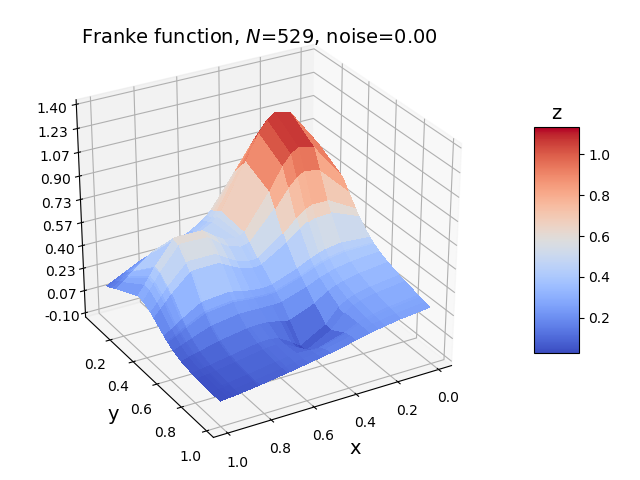
\includegraphics[scale=0.6]{../figures/task_a/surf_franke_N529_nf23_p5_noise0.00_seed4155.png}
	\caption{Example of the Franke function with no noise, with 529 randomly drawn points where $x,y \in [0,1]$.}
	\label{fig:franke_nonoise}
\end{figure}
%
We start the regression analysis by performing the OLS method on the data set. Table \ref{tab:franke_a} shows the MSE and R2 score for the train and test set where $p=5$, $N=529$. For this polynomial degree, both the training and test set shows good results, indicating that there is no significant overfitting.
\begin{table}[H]
  \centering
  \caption{Mean squared error and R2 score for the Franke function training and test set when $p=5$, $N=529$, and noise $\sigma = 0.05$}
  \label{tab:franke_a}
  \begin{tabular}{c|c|c}
    Data set & MSE & R2\\\hline
    train & 0.003334 & 0.949904\\
    test & 0.004674 & 0.929855
    \end{tabular}
\end{table}
The 95\% confidence intervals for $\beta_{\text{OLS}}$ is shown in figure \ref{fig:confbetaOLS}, with the same parameters. The confidence intervals are quite close to the coefficients, which makes sense given the MSE and R2 scores we found earlier.
\begin{figure}[H]
	\centering
	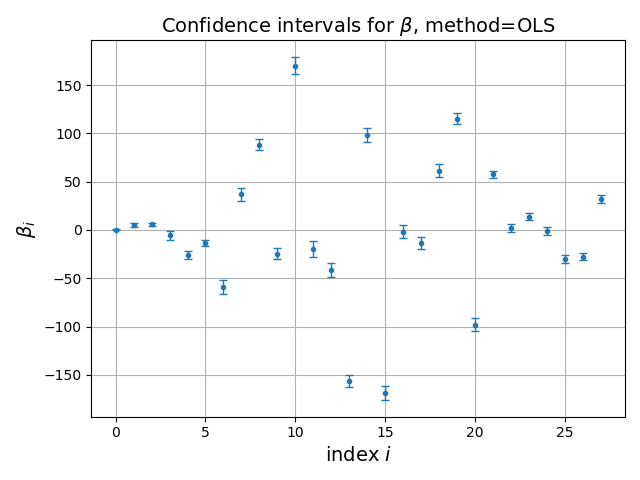
\includegraphics[scale=0.5]{../figures/task_a/beta_conf_int_OLS_N529_nf23_p6_noise0.05_seed4155_beta28.png}
	\caption{95\% confidence intervals for the regression coefficients $\beta_{\text{OLS}}$ for $p=6$, $N=529$, and noise $\sigma=0.05$.}
	\label{fig:confbetaOLS}
\end{figure}
To study how the model is affected by the degree $p$, we study the bias-variance trade-off by employing the Bootstrap resampling method. Now, we will be studying all three regression methods, OLS, Ridge and Lasso to make comparing easier. 
Figure \ref{fig:bias_var} shows the bias-variance trade-off for all three methods, with the Ridge and Lasso ones corresponding to the $\lambda$ that gave the lowest MSE. We see that for the OLS, once we go beyond $p=7$, the error and variance skyrockets. For Ridge and Lasso however, everything is fairly stable for $p>5$. This shows the effect of the regularization parameter $\lambda$, keeping the variance from exploding, and avoiding overfitting.
\begin{figure}[H]
  \centering
  \begin{subfigure}{0.49\textwidth}
    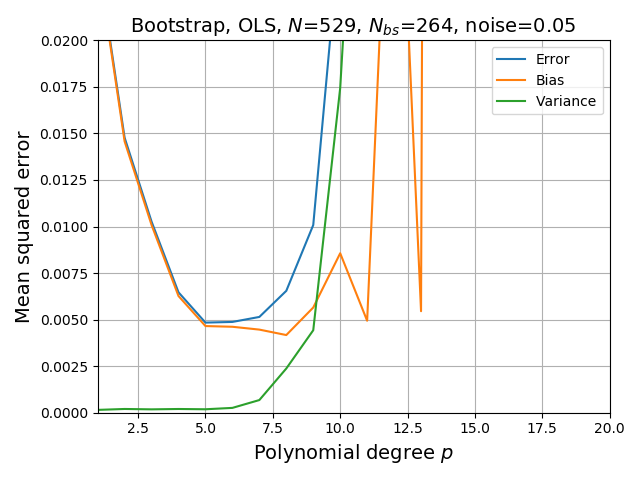
\includegraphics[scale=0.45]{../figures/task_b/bias_variance_N529_pmax20_nlamb1_noise0.05_seed4155_OLS_boot_Nbs264.png}
    \caption{OLS}
  \end{subfigure}
  \begin{subfigure}{0.49\textwidth}
    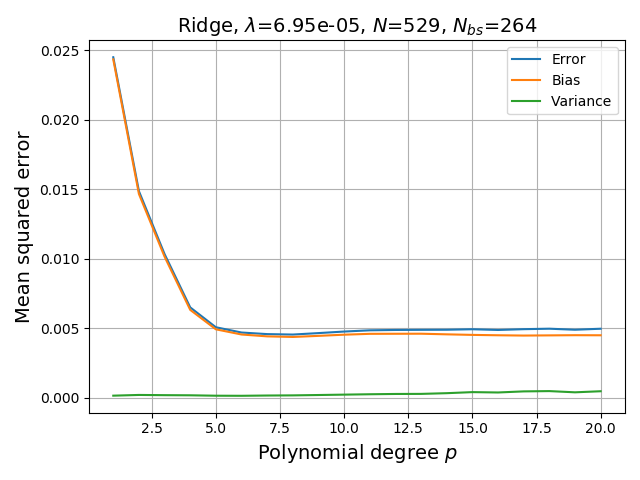
\includegraphics[scale=0.45]{../figures/task_d/bias_variance_N529_pmax20_nlamb20_noise0.05_seed4155_Ridge_boot_Nbs264_opt1.png}
    \caption{Ridge}
  \end{subfigure}\\
  \begin{subfigure}{0.49\textwidth}
    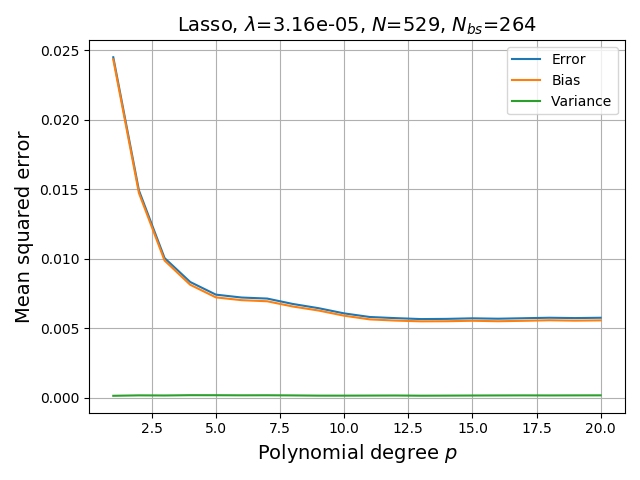
\includegraphics[scale=0.45]{../figures/task_e/bias_variance_N529_pmax20_nlamb15_noise0.05_seed4155_Lasso_boot_Nbs264_opt1.png}
    \caption{Lasso}
  \end{subfigure}
  \caption{Bias-variance plots for OLS, Ridge, and Lasso regression, where $N=529$, $\sigma = 0.05$ and $N_{\text{bs}} = N/2$. The best-fit hyperparameter for Ridge was found to be $\lambda = 2.98\cdot10^{-5}$, and $\lambda = 3.16\cdot10^{-5}$ for Lasso.}
  \label{fig:bias_var}
\end{figure}
Figure \ref{fig:app_Nbs} in appendix \ref{app:Frankeplots} shows how the OLS results depend on the number of bootstraps. Also in the appendix, figure \ref{fig:beta_ridge} shows the 95\% confidence intervals of $\beta$ for Ridge regression, which compared to the OLS confidence intervals shown in figure \ref{fig:confbetaOLS} appear to be slightly larger.\\\\
Before looking closer at the hyperparameters $\lambda$, we look at the results from the $k$-fold Cross-validation. Figure \ref{fig:train_test_franke} shows the difference between the training and test MSE for all regression methods and both Bootstrap and Cross-validation. We see that CV gives very similar results to the Bootstrap, with some discrepancies. For OLS, the test MSE starts shooting up a lot later than for the Bootstrap results. For Ridge, the test MSE lies a lot closer to the training set up until $p=15$, where it starts going slightly up. Finally, Lasso in general is closer to the training MSE.
\begin{figure}[H]
  \centering
  \begin{subfigure}{0.49\textwidth}
    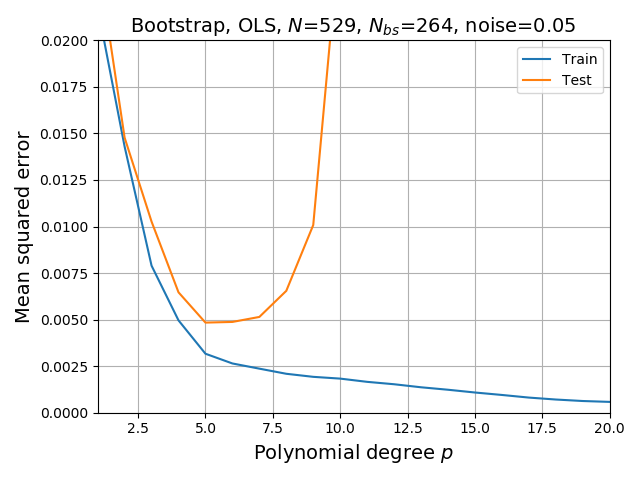
\includegraphics[scale=0.45]{../figures/task_b/MSE_train_test_Bootstrap_train_test_N529_pmax20_nlamb1_noise0.05_seed4155_OLS_boot_Nbs264.png}
    \caption{OLS - Bootstrap}
  \end{subfigure}
  \begin{subfigure}{0.49\textwidth}
    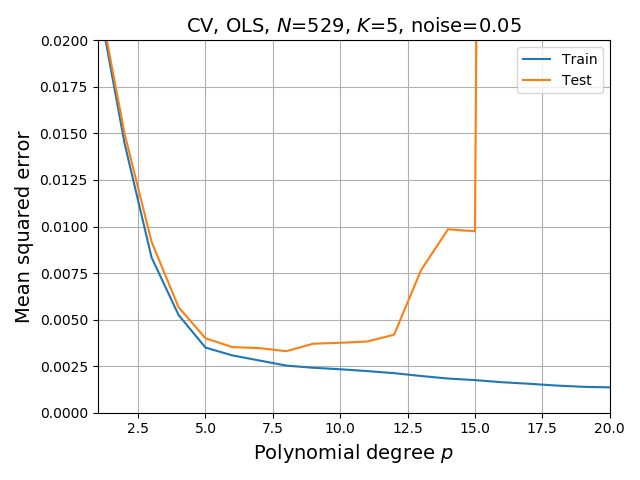
\includegraphics[scale=0.45]{../figures/task_b/MSE_train_test_CV_train_test_N529_pmax20_nlamb1_noise0.05_seed4155_OLS_cv_k5.png}
    \caption{OLS - Cross-validation}
  \end{subfigure}\\
  \begin{subfigure}{0.49\textwidth}
    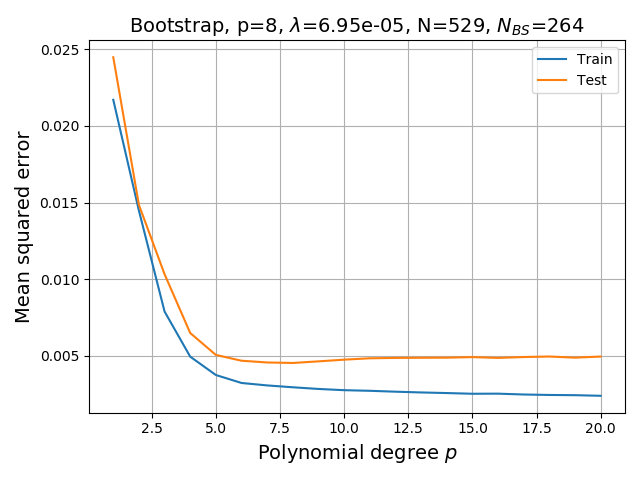
\includegraphics[scale=0.45]{../figures/task_d/MSE_train_test_Bootstrap_N529_pmax20_nlamb20_noise0.05_seed4155_Ridge_boot_Nbs264_opt1.png}
    \caption{Ridge - Bootstrap}
  \end{subfigure}
  \begin{subfigure}{0.49\textwidth}
    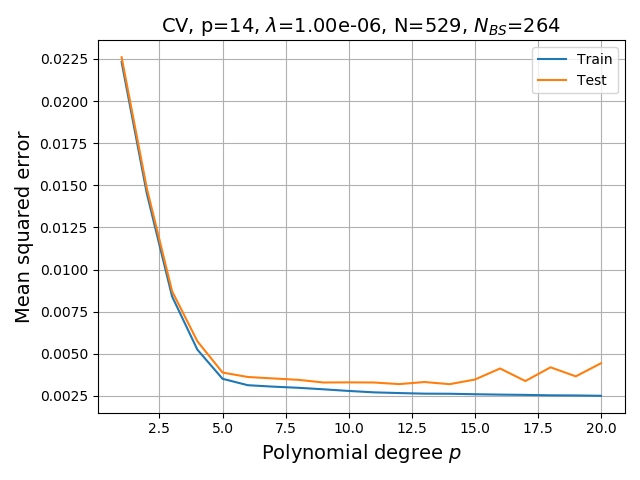
\includegraphics[scale=0.45]{../figures/task_d/MSE_train_test_CV_N529_pmax20_nlamb20_noise0.05_seed4155_Ridge_cv_k5_opt1.png}
    \caption{Ridge - Cross-validation}
  \end{subfigure}\\
  \begin{subfigure}{0.49\textwidth}
    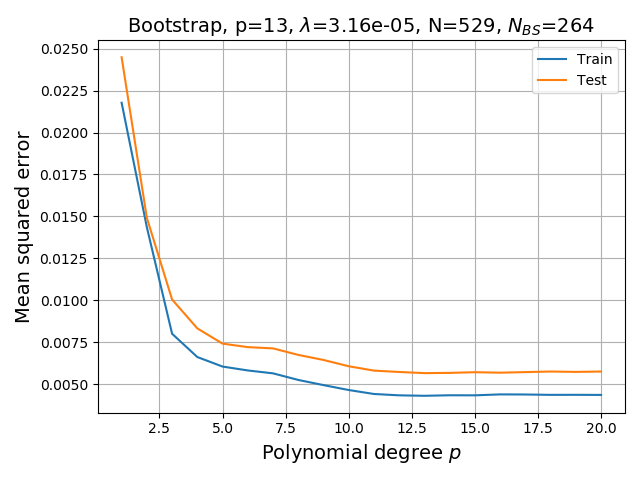
\includegraphics[scale=0.45]{../figures/task_e/MSE_train_test_Bootstrap_N529_pmax20_nlamb15_noise0.05_seed4155_Lasso_boot_Nbs264_opt1.png}
    \caption{Lasso - Bootstrap}
  \end{subfigure}
  \begin{subfigure}{0.49\textwidth}
    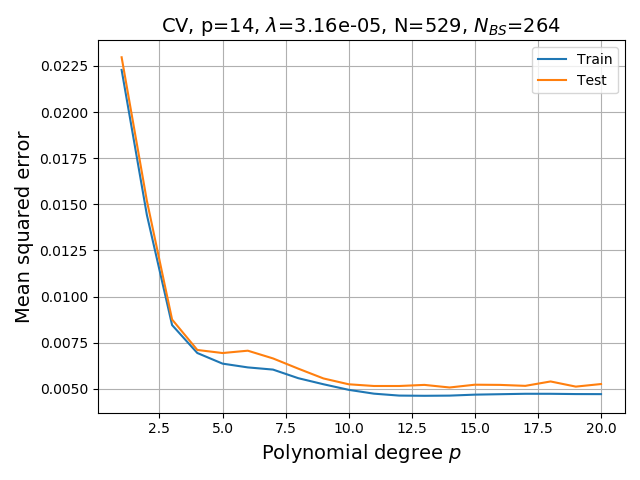
\includegraphics[scale=0.45]{../figures/task_e/MSE_train_test_CV_N529_pmax20_nlamb15_noise0.05_seed4155_Lasso_cv_k5_opt1.png}
    \caption{Lasso - Cross-validation}
  \end{subfigure}\\  
  \caption{Bias-variance plots for OLS, Ridge, and Lasso regression, where $N=529$, $\sigma = 0.05$ and $N_{\text{bs}} = N/2$. The best-fit hyperparameter for Ridge was found to be $\lambda = 2.98\cdot10^{-5}$, and $\lambda = 3.16\cdot10^{-5}$ for Lasso. The $p$-value on the Ridge + CV panel should have been the $p$-value corresponding to the minimum MSE value, but for some reason it is wrong.}
  \label{fig:train_test_franke}
\end{figure}
One way of looking at the hyperparameters would be to look at the heat map from all the values of $p$ and $\lambda$ that we used. Figure \ref{fig:franke_heatmap} shows the MSE heat map for Ridge and Lasso using Bootstrap. Heat maps for the bias, variance, and MSE from CV can be found in the Github repository \cite{Github1}. It is clear that the model prefers lower $\lambda$, though for high model complexity/polynomial degree a slightly higher $\lambda$ is preferred. While for Ridge, a large amount of the $\lambda$s give a good result, for Lasso the MSE almost always increase as $\lambda$ is increased. 
\begin{figure}[H]
  \centering
  \begin{subfigure}{0.49\textwidth}
    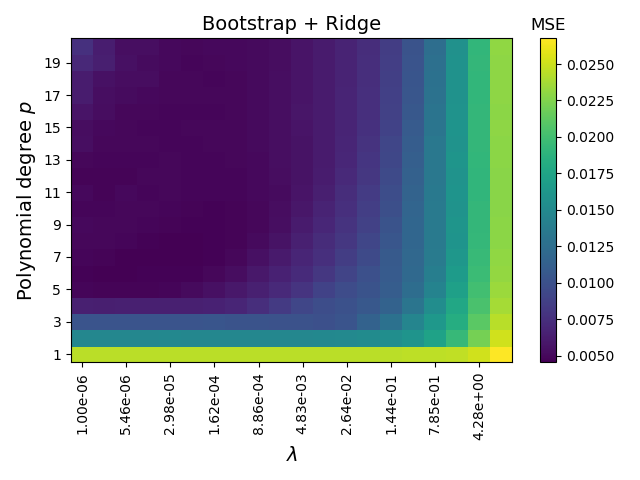
\includegraphics[scale=0.45]{../figures/task_d/heatmap_bs_error_N529_pmax20_nlamb20_noise0.05_seed4155_Ridge_boot_Nbs264.png}
    \caption{Ridge}
  \end{subfigure}
  \begin{subfigure}{0.49\textwidth}
    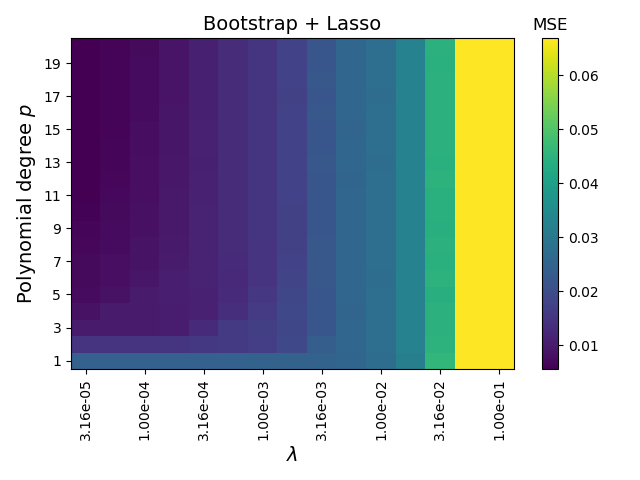
\includegraphics[scale=0.45]{../figures/task_e/heatmap_bs_error_N529_pmax20_nlamb15_noise0.05_seed4155_Lasso_boot_Nbs264.png}
    \caption{Lasso}
  \end{subfigure}
  \caption{Heat maps showing the MSE plotted against polynomial degree $p$ and the hyperparameter $\lambda$ for both Ridge and Lasso, using Bootstrap resampling.}
  \label{fig:franke_heatmap}
\end{figure}
Figure \ref{fig:franke_lambdap} shows $\lambda_{\text{min}}$ plotted against $p$ for both Ridge and Lasso where $\lambda_{\text{min}}$ is the $\lambda$ corresponding to the lowest MSE for that polynomial degree. This is done both for Bootstrap and Cross-validation. For Ridge and Bootstrap, the optimal $\lambda$ varies quite a bit for each value of $p$, while for CV, it stays at the lowest value for $p \in [8, 12]$, where there is a peak in the Bootstrap. The axes are slightly different, so plotting them on top of each other would have been interesting.\\\\
For Lasso, the $\lambda$ value drops down to the lowest value at $p\sim3-4$ for both Bootstrap and CV, staying there until the end. This shows that we probably should have tried running with even lower values. Sadly, running with the same starting point $\lambda = 1\cdot10^{-6}$ as Ridge caused a lot of convergence errors, and took extremely long time without finishing.
\begin{figure}[H]
  \centering
  \begin{subfigure}{0.49\textwidth}
    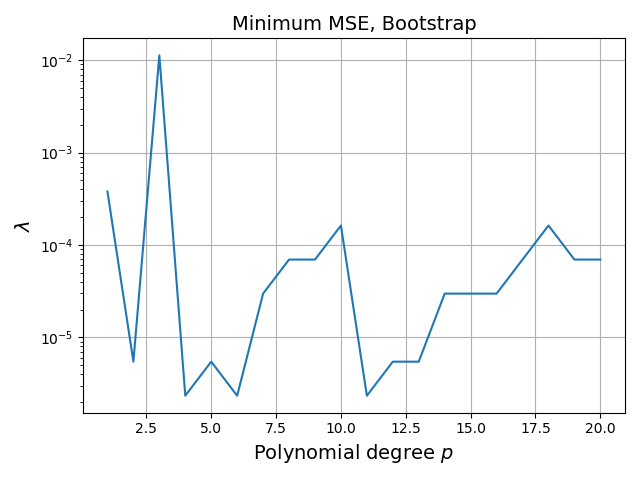
\includegraphics[scale=0.45]{../figures/task_d/degree_lambda_N529_pmax20_nlamb20_noise0.05_seed4155_Ridge_boot_Nbs264.png}
    \caption{Ridge - Bootstrap}
  \end{subfigure}
  \begin{subfigure}{0.49\textwidth}
    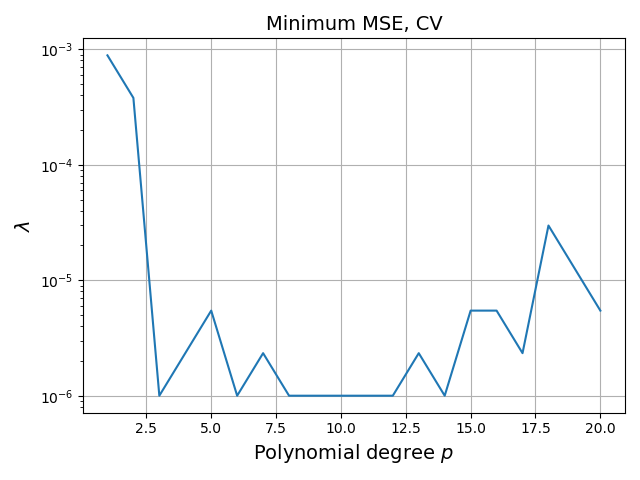
\includegraphics[scale=0.45]{../figures/task_d/degree_lambda_N529_pmax20_nlamb20_noise0.05_seed4155_Ridge_cv_k5.png}
    \caption{Ridge - Cross-validation}
  \end{subfigure}\\
  \begin{subfigure}{0.49\textwidth}
    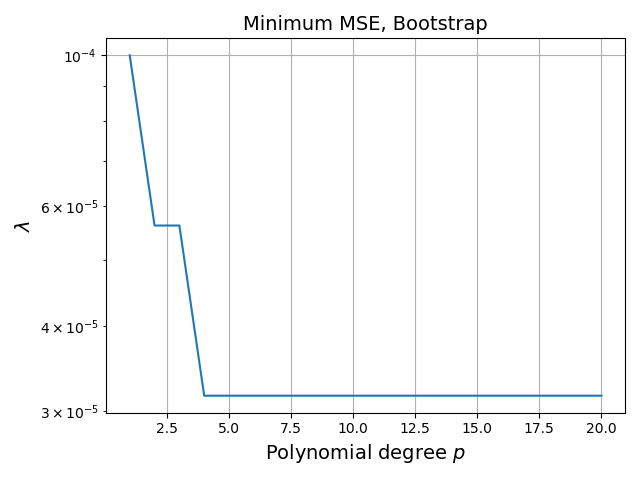
\includegraphics[scale=0.45]{../figures/task_e/degree_lambda_N529_pmax20_nlamb15_noise0.05_seed4155_Lasso_boot_Nbs264.png}
    \caption{Lasso - Bootstrap}
  \end{subfigure}
  \begin{subfigure}{0.49\textwidth}
    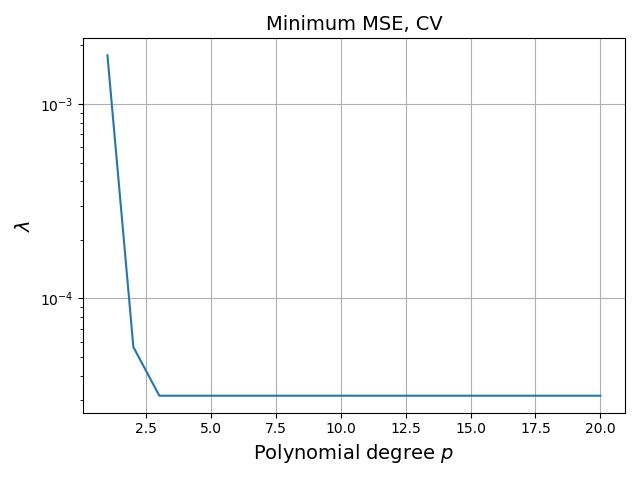
\includegraphics[scale=0.45]{../figures/task_e/degree_lambda_N529_pmax20_nlamb15_noise0.05_seed4155_Lasso_cv_k5.png}
    \caption{Lasso - Cross-validation}
  \end{subfigure}
  \caption{Hyperparameter $\lambda$ plotted against polynomial degree $p$ for Ridge/Lasso regression with Bootstrap/Cross-validation. The $\lambda$ value corresponds to the one that gives the lowest MSE value at the given $p$.}
  \label{fig:franke_lambdap}
\end{figure}
Finally, table \ref{tab:best_fit_franke} shows the best-fit parameters $p$ and $\lambda$ for each of the three regression methods, and for each of the resampling methods. For both Bootstrap and Cross-validation, Ridge regression seems to be the best option, while Lasso seems to be the worst. Part of the reason why Lasso performs the worst here could be because of the $\lambda$-values not being low enough as explained earlier, causing us to miss the best fit for Lasso. OLS however performs very close to Ridge, especially in the Cross-validation, and it is the fastest regression method, while Lasso can be extremely slow as there is no analytical solution. That said, both Ridge and Lasso have a significant advantage when it comes to stability. As shown with both the bias-variance trade-off and train-test plots, Ridge and Lasso has a much wider range of parameters that give good results, as the hyperparameter suppresses the overfitting problem with OLS.
\begin{table}[H]
  \centering
  \caption{The best-fit parameters for OLS, Ridge and Lasso regression given the lowest MSE value. First three columns is the Bootstrap, last three is Cross-validation}
  \label{tab:best_fit_franke}
  \begin{tabular}{c|c|c|c||c|c|c}
    Reg. method & p (BS)& $\lambda$ (BS) & MSE (BS) & p (CV) & $\lambda$ (CV) & MSE (CV) \\\hline
    OLS & 5 & - & $4.84\cdot10^{-3}$ & 8 & - & $3.30\cdot10^{-03}$\\
    Ridge & 8 & $6.95\cdot10^{-5}$ & $4.55\cdot10^{-3}$ & 15 & $5.46\cdot10^{-6}$ & $3.28\cdot10^{-3}$\\
    Lasso & 13 & $3.16\cdot10^{-5}$ &$5.67\cdot10^{-3}$ & 14 & $3.16\cdot10^{-5}$ & $5.08\cdot10^{-3}$
    \end{tabular}
\end{table}
Before moving on to the terrain data, to point out that for some reason the $p$ and $\lambda$ values present in the title of figure \ref{fig:train_test_franke} for the CV+Ridge panel specifically for some reason is incorrect. Quite a bit of time was spent looking at the code and output files without understanding why that one specifically is wrong.
\subsection{Terrain data}
\subsection{Further discussion} \label{sub:discussion}
\red{maybe refer to how i checked bootstrap compared SKL/OLS, and lecture notes. CV skl vs ols?}
\red{figure out sectioning}
Mention bootstrap and how at higher degrees, some samples jst
The number of outliers, as in where predicted values values are very far from test data gets higher the higher polynomial degree, and causes the bias to shoot up for some reason Despite resampling, it appears to be the same indices that give the fucked up value
In the $n=1024$, $nbs=2$, $p=15$, $noise=0.05$ case, index 196 has a y\_pred of 19 and 25ish setting it to the value of 195 gives a max value of y\_pred of $1.2$isho why the hell does one row get so incredibly messed up?????
And why is it extremely wrong in both bootstraps despite having shuffled everything?
Replacing X\_test$[196]$ with X\_test$[195]$ "removes" the outlier, while just changing y\_test$[196]$ does nothing 
\\\\
Maybe related to RNG and seed?
WATHa haw results are weird with minimum in files
%%%%%%%%%%%%%%%%%%%%%%%%%%%%%%%%%%%%%%%%%%%%%%%%%%%%%%%%%%%%%%%%%%%%%%%%%%%%%%%%%%%%%%%%%%
%%%%%%%%%%%%%%%%%%%%%%%%%%%%%%%%%%%%%%%%%%%%%%%%%%%%%%%%%%%%%%%%%%%%%%%%%%%%%%%%%%%%%%%%%%
\section{Conclusion} \label{chap:conclusion}
Introduce why we set out, then explain results

no idea why problems are, but the way the code is structured, sadly makes debugging slow.
%%%%%%%%%%%%%%%%%%%%%%%%%%%%%%%%%%%%%%%%%%%%%%%%%%%%%%%%%%%%%%%%%%%%%%%%%%%%%%%%%%%%%%%%%%
%%%%%%%%%%%%%%%%%%%%%%%%%%%%%%%%%%%%%%%%%%%%%%%%%%%%%%%%%%%%%%%%%%%%%%%%%%%%%%%%%%%%%%%%%%
\bibliography{references}
%%%%%%%%%%%%%%%%%%%%%%%%%%%%%%%%%%%%%%%%%%%%%%%%%%%%%%%%%%%%%%%%%%%%%%%%%%%%%%%%%%%%%%%%%%
%%%%%%%%%%%%%%%%%%%%%%%%%%%%%%%%%%%%%%%%%%%%%%%%%%%%%%%%%%%%%%%%%%%%%%%%%%%%%%%%%%%%%%%%%%
\appendix
\section*{Appendix} \label{chap:appendix}
%\section{Appendix} \label{chap:appendix}
\section{Data sets} \label{app:datasets}
\subsection{Franke function} \label{app:Franke}
The Franke function as given in \cite{Franke}
\begin{align*}
	f(x,y) &= \frac{3}{4}\exp\bigg(-\frac{(9x-2)^2}{4} - \frac{(9y-2)^2}{4}\bigg)
	+\frac{3}{4}\exp\bigg(-\frac{(9x+1)^2}{49} - \frac{(9y+1)^2}{10}\bigg)\\
	&+\frac{1}{2}\exp\bigg(-\frac{(9x-7)^2}{4} - \frac{(9y-3)^2}{4}\bigg)
	-\frac{1}{5}\exp\big(-(9x-4)^2 - (9y-7)^2\big)
\end{align*}
where $x,y \in [0, 1]$.

\subsection{Terrain data} \label{app:terrain}
\begin{figure}[H]
	\centering
	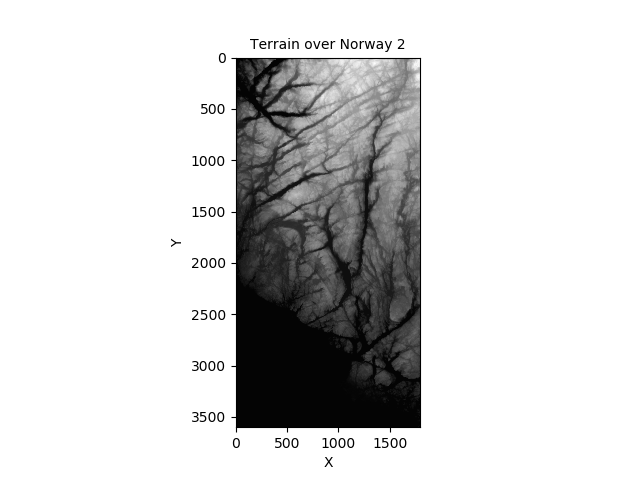
\includegraphics[scale=0.8]{../figures/task_f/entire_map.png}
	\caption{Plot of the entire terrain map in \texttt{SRTM\_data\_Norway\_3.tif}. Map is over a region south-east in Norway (Vestfold og Telemark, Viken). Coordinates $(x,y) = (1100, 3000)$ correspond to the location of the city Skien.}
	\label{fig:entiremap}
\end{figure}

\section{Testing and verifying methods} \label{app:testing}

\section{Franke function plots} \label{app:Frankeplots}
\begin{figure}[H]
  \centering
  \begin{subfigure}{0.49\textwidth}
    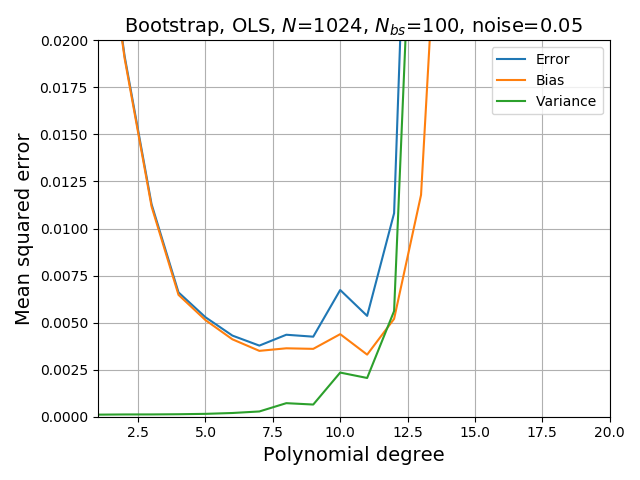
\includegraphics[scale=0.45]{../figures/task_b/bias_variance_N1024_pmax20_nlamb1_noise0.05_seed4155_OLS_boot_Nbs100.png}
    \caption{$N_{\text{bs}} = 100$}
  \end{subfigure}
  \begin{subfigure}{0.49\textwidth}
    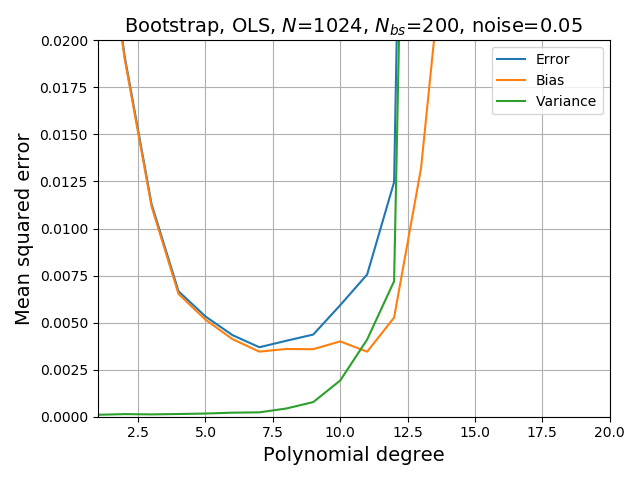
\includegraphics[scale=0.45]{../figures/task_b/bias_variance_N1024_pmax20_nlamb1_noise0.05_seed4155_OLS_boot_Nbs200.png}
    \caption{$N_{\text{bs}} = 200$}
  \end{subfigure}\\
  \begin{subfigure}{0.49\textwidth}
    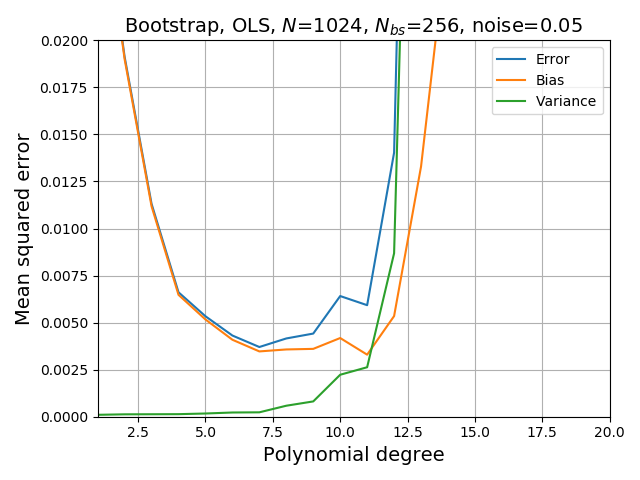
\includegraphics[scale=0.45]{../figures/task_b/bias_variance_N1024_pmax20_nlamb1_noise0.05_seed4155_OLS_boot_Nbs256.png}
    \caption{$N_{\text{bs}} = 256$}
  \end{subfigure}
  \begin{subfigure}{0.49\textwidth}
    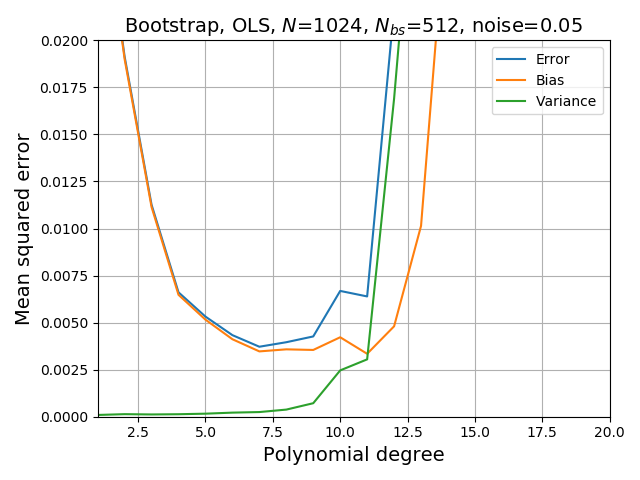
\includegraphics[scale=0.45]{../figures/task_b/bias_variance_N1024_pmax20_nlamb1_noise0.05_seed4155_OLS_boot_Nbs512.png}
    \caption{$N_{\text{bs}} = 512$}
  \end{subfigure}
  \caption{Bias-variance plots for OLS where the number of bootstraps $N_{\text{bs}}$ is varied. $N=1024$, $\sigma=0.05$. In general, all four produce very similar results.}
  \label{fig:app_Nbs}
\end{figure}

\begin{figure}[H]
	\centering
	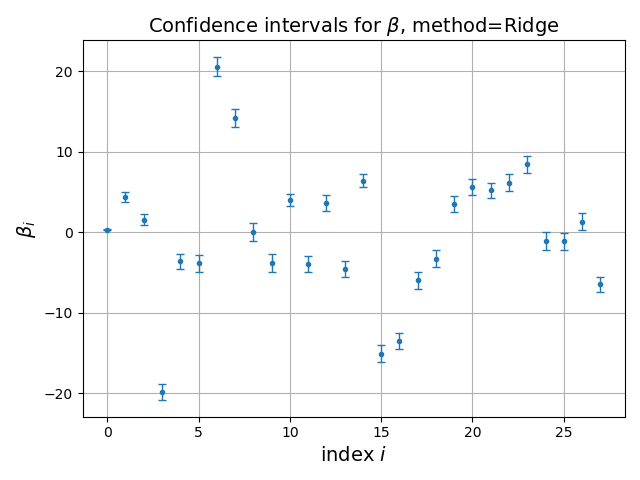
\includegraphics[scale=0.5]{../figures/task_d/beta_conf_int_Ridge_N529_pmax20_nlamb20_noise0.05_seed4155_beta28.png}
	\caption{95\% confidence intervals for the regression coefficients $\beta_{\text{Ridge}}$ for $p=6$, $N=529$, and noise $\sigma=0.05$.}
	\label{fig:beta_ridge}
\end{figure}
\section{Terrain data plots} \label{app:terrainplots}
%\subsubsection{Hyperpar

\end{document}